\documentclass[amsmath,amssymb,twocolumn,superscriptaddress]{revtex4-1}

\usepackage{graphicx}% Include figure files
\usepackage{dcolumn}% Align table columns on decimal point
\usepackage{bm}% bold math
\usepackage[detect-all]{siunitx}
\usepackage{hyperref}% add hypertext capabilities
\usepackage{xr}

\begin{document}                  % DO NOT DELETE THIS LINE

\title{An introduction to classical molecular dynamics simulation for experimental scattering users}

\author{A.~R. McCluskey}
\email{a.r.mccluskey@bath.ac.uk/andrew.mccluskey@diamond.ac.uk}
\affiliation{Department of Chemistry, University of Bath, Claverton Down,
Bath, BA2 7AY, UK}
\affiliation{Diamond Light Source, Harwell Campus, Didcot, OX11 0DE, UK}

\author{J. Grant}
\affiliation{Computing Services, University of Bath, Claverton Down, Bath, BA2 7AY, UK}

\author{A.~R. Symington}
\affiliation{Department of Chemistry, University of Bath, Claverton Down,
Bath, BA2 7AY, UK}

\author{T.~Snow}
\affiliation{Diamond Light Source, Harwell Campus, Didcot, OX11 0DE, UK}
\affiliation{School of Chemistry, University of Bristol, Bristol, BS8 1TS, UK}

\author{J.~Doutch}
\affiliation{ISIS Facility, Rutherford Appleton Laboratory, STFC, Chilton, Didcot, OX11 0QX, UK}

\author{B.~J. Morgan}
\email{b.j.morgan@bath.ac.uk}
\affiliation{Department of Chemistry, University of Bath, Claverton Down,
Bath, BA2 7AY, UK}

\author{S.~C. Parker}
\affiliation{Department of Chemistry, University of Bath, Claverton Down,
Bath, BA2 7AY, UK}

\author{K.~J. Edler}
\affiliation{Department of Chemistry, University of Bath, Claverton Down,
Bath, BA2 7AY, UK}

\date{\today}

\begin{abstract}
\noindent Classical molecular dynamics simulations are a common component of multi-modal analyses from scattering measurements, such as small-angle scattering and diffraction.
Users of these techniques often have no formal training in the theory and practice of molecular dynamics simulation, leading to the possibility of these being treated as a ``black box'' analysis technique.
This work discusses an open educational resource designed to introduce classical molecular dynamics to users of scattering methods.
This resource comes in the form of a series of interactive web pages, which can be run from any device with internet connectivity.
We present a general introduction to topics including classical simulation, potential model parameterisation and molecular dynamics simulation.
We then discuss typical sources of error in classical molecular dynamics simulations, before considering some of the approaches to using simulations in the analysis of scattering data.
\end{abstract}

\maketitle                        % DO NOT DELETE THIS LINE

\section{Introduction}

\noindent The use of molecular dynamics simulations to help analyse experimental data, particularly from small-angle scattering and diffraction, has grown significantly over the past ten years \cite{pan_molecular_2012,boldon_review_2015,hub_interpreting_2018,ivanovic_temperature-dependent_2018,east_structural_2016,wall_conformational_2014,wall_internal_2018,satoh_multiple_2015}.
Figure \ref{fig:growth} shows the percentage of small-angle scattering publications that mention molecular dynamics in recent years, reaching more than \SI{20}{\percent} of small-angle scattering articles published in 2018.

Users of scattering and diffraction techniques often have backgrounds in experimental science, with little or no formal training in the theory or practice of computational modelling.
This can lead to molecular dynamics simulations being used as a ``black box'', with little understanding of the underlying methodologies, or consideration of possible sources of erroneous results.
The use of molecular simulations without at least some understanding of the techniques can lead to the unintended inclusion of severe, systematic errors.
The challenge of enabling researchers to use molecular dynamics simulation in their analysis of scattering data, while reducing this risk of modelling errors, has lead to the development of software tools, such as WAXSiS and SASSIE \cite{chen_validating_2014,knight_waxsis_2015,perkins_atomistic_2016}, that present easy-to-use, graphical, web-based interfaces to operate the software.

A complementary strategy to help avoid researchers inadvertently using erroneous simulation results is targetted educational resources and activities, such as lectures or workshops that introduce molecular simulation to audiences of scattering and diffraction users.
One example is the annual ISIS Neutron Training Course, which includes a module entitled ``An Introduction to Molecular Dynamics for Neutron Scattering''.
This covers the fundamentals of classical molecular dynamics simulation, presents applications of these methods in neutron science, and allows students to gain practical experience with the SASSIE software package \cite{perkins_atomistic_2016}.

%
\begin{figure}
\label{fig:growth}
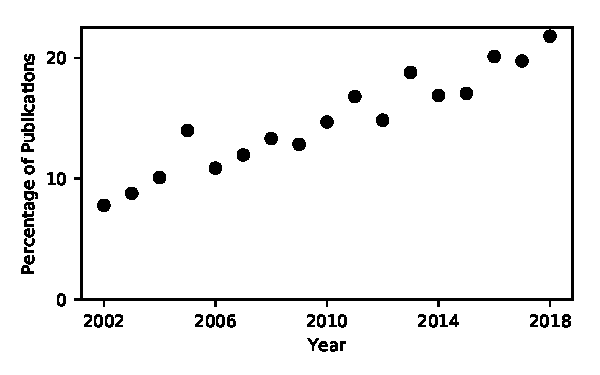
\includegraphics[width=0.48\textwidth]{figures/chem_data_py.pdf}
\caption{The annual percentage of publications that mention ``small angle scattering'' that also mention ``molecular dynamics'', determined from the numbers of matching Google Scholar results.}
\end{figure}
%

While lectures and workshops are a valuable approach to education and training, participation can be limited due to difficulties attending in person (due to location or cost) or physical limits on student numbers.
An alternative educational medium gaining popularity within scientific and engineering communities is technology-enhanced open educational resources (OERs).
These are courses, lectures, or learning resources published online that are freely available for use by anyone. In addition to their broad accessibility, these resources adopt permissive, ``open'' copyright licences that permit their use in the ``5R activities'': retain, reuse, revise, remix, and redistribute \cite{wiley_open_2018}.
The act of publishing a resouce as an OER increases its reach and cumulative impact, because others may take it for immediate use in their own teaching, or freely modify the material to suit their needs.
The Jupyter Notebook framework \cite{kluyver_jupyter_2016} has become a popular platform for OERs that teach computational skills, because it allows authors to include instructional text, images, and other media, alongside executable code examples, in an example of ``literate programming'' \cite{knuth_literate_1984}.
This format encourages students to directly interact with the code by editing and rerunning this within the source document \cite{barba_cybertraining_2017}.

In this article, we present an online, open-source, interactive learning resource aimed to introduce members of the scattering and diffraction community to molecular dynamics simulations.
This open educational resource is comprised of six lessons that introduce classical molecular dynamics methods, and show how these can be used in the context of scattering in a multi-modal analysis fashion
To provide simple, but computationally ``real'' examples of simulations, we use the open-source Python library pylj \cite{mccluskey_pylj_2018} to demonstrate visually and programmatically the conceptual relationships between these two techniques.
Here, we discuss the structure of the resource and describe how a student\footnote{In this work \emph{the student} refers to anyone working through the OER, regardless of career position.} may get the most from the resource.

\section{Assumed prior knowledge}

The OER, entitled \emph{``The interaction between simulation and scattering''} makes use of the Python programming language, which allows interactive examples of the mathematical and algorithm content to be included.
A result of this is that to be able to fully utilise the resource some knowledge of, or willingness to learn, Python is required.
However, we have attempted to develop the resource in such a fashion that an in-depth knowledge of Python is not required.
It is anticipated that the users of this resource would have some familiarity with undergraduate level chemistry or physics, alongside a commensurate understanding of mathematics.
This is particularly important when considering the nature, and chemical rationale, of classical interaction potentials.

\section{Resource construction}

The resource is currently available online, at \url{http://pythoninchemistry.org/sim_and_scat}.
These webpages were written as a series of Jupyter Notebooks and Markdown files, which were then compiled using the \texttt{jupyter-book} tool \cite{lau_jupyter/jupyter-book_2019}.
This system allows Python code blocks to be included alongside the textual content, providing algorihtmic details whilst also facilitating interactivity, though both Thebelab and BinderHub integrations \cite{ragan-kelley_minrk/thebelab_2019,ragan-kelley_jupyterhub/binderhub_2019,jupyter_binder_2018}.
Interacting with the resource in this fashion will aloow the student to either run the Python code directly in the resource interface (Thebelab), or easily launch a MyBinder window to more intensive visualisations (such as pylj).
We believe that the interactive nature of the resource will facilitate understanding allowing the students to gain more than would be obtained from a traditional lecture or handout material \cite{knuth_literate_1984}.

The resource is provided under a CC-BY-4.0 license \cite{noauthor_creative_2019} and builds on the growing library of open educational resources.
The open-source nature of this license means that anyone may use the material to enhance their own educational platform and experts in the field may contribute to improving the resource.
The source code for the resource is available at \url{https://github.com/pythoninchemistry/sim_and_scat} \cite{mccluskey_pythoninchemistry/sim_and_scat_2019}.

\section{Resource outline}

The resource follows a simple outline to introduce important aspects of molecular dynamics simulations.
Code blocks are used to gradually build up the student's understanding of the various concepts.

\subsection{Home}

The welcome page introduces the resource and gives the student information about how the resource may be used, including details of Thebelab and BinderHub integration.
Furthermore, this page gives information about the use and sharing of the content of the resource including details of the license.
This page also includes an authors and contributors list.

\subsection{Classical methods}

Following the introduction, concepts relating broadly to classical simulation methods are introduced.
This includes the functional nature of potential modelling and gives some examples, such as the Lennard-Jones and Buckingham potential models \cite{lennard-jones_determination_1924,buckingham_classical_1938}.
The potential model parameterisation is briefly covered including the use of higher accuracy quantum mechanical calculations to do so.
The presence of off-the-shelf, general potential models are discussed; with particular attention paid to the caveat that they may still require system specific optimisations.
Finally, we mention mixing rules; again discussing the possible problems that a user may encounter related to system specificity.

\subsection{Molecular dynamics}

Building on the classical potential model methods the student is then presented with molecular dynamics.
This is shown by using different aspects for the method to gradually build up a one-dimensional molecular dynamics simulation using NVE (Number, Volume and Energy) ensembles, the Velocity-Verlet algorithm and the Lennard-Jones potential model \cite{swope_computer_1982,lennard-jones_determination_1924}.
This is introduced in terms of Newton's laws of motion and the generalised equations of motion, which should be familiar to most students.
Finally, different importance considerations for molecular dynamics simulations are described including ensembles, the potential cut-off, and periodic boundary conditions.

\subsection{\texttt{pylj} and the interaction with scattering}

The final aspect of the resource is to utilise a molecular dynamics simulation to understand some scattering profiles.
This is achieved using the open-source \texttt{pylj} package \cite{mccluskey_pylj_2018}, which allows for a two-dimensional simulation or argon particles, interacting through a Lennard-Jones potential, to be performed.
The student is first shown a working \texttt{pylj} simulation and invited to interact with the simulation and the custom plotting functionality of \texttt{pylj}.
In the final lessons, a formulation of the Debye equation \cite{debye_zerstreuung_1915} is given and the student is invited to observe the effect of simulation temperature on the resulting scattering profile.
There is mention of other, faster, algorithms for the determination of scattering profiles, such as the Fibonacci sequence or Golden Vectors methods \cite{svergun_solution_1994,watson_rapid_2013}.

\section{Future outlook}

In the future, we hope that the nature of the material, as an OER, will promote interest from other parties towards reuse, and remixing the material.
Furthermore, we hope to implement this material within training at the ISIS Neutron and Muon Source as well as Diamond Light Source.
Finally, it is hoped, \textit{via} student and community feedback, that the improvement of implementation, materials, and general pedagogy of the resource can be achieved, driving up the quality and depth of molecular dynamics analyses performed on results obtained from scattering and diffraction measurements.

\section{Author contributions}

The open education resource was developed, and the manuscript written, by A. R. M. with input from all authors.

\begin{acknowledgements}
A. R. M. is grateful to the University of Bath and Diamond Light Source for co-funding a studentship (Studentship No. STU0149).
B. J. M. acknowledges support from the Royal Society (Grant No. UF130329).
\end{acknowledgements}

\bibliography{bib.bib}


\end{document}                    % DO NOT DELETE THIS LINE
